% !TEX program = xelatex
\documentclass[a4paper,11pt]{article}
% Compiler avec XeLaTeX ou LuaLaTeX (requis par la page de garde)
\usepackage{fontspec}
\usepackage[french]{babel}
\usepackage{amsmath}
\usepackage{graphicx}
\usepackage{tikz}
\usetikzlibrary{calc}
\usepackage{setspace}
\usepackage{xurl}

\begin{document}
% --- Page de garde (contenu du document) ---
%
% =====================
% Prérequis (important)
% =====================
% Ce fichier est inclus depuis Rapport.tex (donc après \begin{document}).
% => Ne PAS mettre de \usepackage ici.
%
% Moteur requis (à cause de \fontspec et des polices TTF):
% - XeLaTeX ou LuaLaTeX
%
% Packages à charger dans le préambule (ex: package.tex):
% - \usepackage{fontspec}   % \fontspec
% - \usepackage{graphicx}   % \includegraphics
% - \usepackage{tikz}       % overlay + placement
%   \usetikzlibrary{calc}   % ([xshift=...,yshift=...])
% - \usepackage{setspace}   % \setstretch
%
% Ressources attendues:
% - FrontPage/tahoma.ttf et FrontPage/tahomabd.ttf
% - Le PDF de fond (voir \FrontPageBackgroundPdf)
% - Le logo entreprise (voir \FrontPageCompanyLogo)


% =====================
% Variables (à modifier)
% =====================

% Debug : mettre à true pour afficher les cadres TikZ.
\newif\ifFrontPageDebug
% \FrontPageDebugtrue
\FrontPageDebugfalse

% Titre (diplôme)
\newcommand{\FrontPageTitle}{Titre centré}

% Titre central (note)
\newcommand{\FrontPageTitleNote}{%
  Il faut respecter le titre definitif au point,
à la virgule et à la majuscule PRES
(titre exact qui paraîtra sur le diplôme)
}

% Noms / date
\newcommand{\FrontPageStudentName}{Prénom NOM}
\newcommand{\FrontPageDefenceDate}{Date}

% Choix de finalité : mettre à true pour A, à false pour B
\newif\ifFrontPageFinalityA
% \FrontPageFinalityAfalse
\FrontPageFinalityAtrue

% Mentors / entreprise
\newcommand{\FrontPageGrammeMentorName}{Prénom NOM}
\newcommand{\FrontPageGrammeMentorPost}{Fonction}
\newcommand{\FrontPageEnterpriseMentorName}{Prénom NOM}
\newcommand{\FrontPageEnterpriseMentorPost}{Fonction}
\newcommand{\FrontPageCompanyName}{Nom}

% =============================
% Constantes (à modifier rarement)
% =============================

% Ressources
\newcommand{\FrontPageBackgroundPdf}{FrontPage/FrontPage_FR.pdf}
\newcommand{\FrontPageFontPath}{FrontPage/}
\newcommand{\FrontPageFontUpright}{tahoma.ttf}
\newcommand{\FrontPageFontBold}{tahomabd.ttf}
\newcommand{\FrontPageCompanyLogo}{FrontPage/company_logo.jpg}

% Bloc haut
\newcommand{\FrontPageHeaderMain}{Travail de Fin d'Études}
\newcommand{\FrontPageHeaderSubtitle}{En vue de l'obtention du grade de}
\newcommand{\FrontPageHeaderDegree}{Master en Sciences de l'Ingénieur Industriel}
\newcommand{\FrontPageHeaderFinalityA}{Industrie}
\newcommand{\FrontPageHeaderFinalityB}{Génie Énergétique Durable}

% Libellés
\newcommand{\FrontPagePresentedBy}{Mémoire présenté par}
\newcommand{\FrontPageDefenceLabel}{Défense publique le}
\newcommand{\FrontPageGrammeMentorLabel}{Tuteur Gramme}
\newcommand{\FrontPageEnterpriseMentorLabel}{Tuteur entreprise}
\newcommand{\FrontPageCompanyLabel}{Société}

% Finalité : résout le texte affiché selon le choix A/B
\newcommand{\FrontPageSelectedFinality}{%
  \ifFrontPageFinalityA
    \FrontPageHeaderFinalityA
  \else
    \FrontPageHeaderFinalityB
  \fi
}

% Mentors : toujours afficher les deux (Gramme + entreprise)
\newcommand{\FrontPageMentorsBlock}{%
  {\bfseries\fontsize{10}{12}\selectfont \FrontPageGrammeMentorLabel}\par
  {\fontsize{10}{12}\selectfont \FrontPageGrammeMentorName}\par
  {\fontsize{10}{12}\selectfont \FrontPageGrammeMentorPost}\par
  \vspace{0.8cm}
  {\bfseries\fontsize{10}{12}\selectfont \FrontPageEnterpriseMentorLabel}\par
  {\fontsize{10}{12}\selectfont \FrontPageEnterpriseMentorName}\par
  {\fontsize{10}{12}\selectfont \FrontPageEnterpriseMentorPost}\par
}

% Mise en page (valeurs de position/taille)
\newcommand{\FrontPageTitleBoxW}{0.7\paperwidth}
\newcommand{\FrontPageTitleBoxH}{6.5cm}
\newcommand{\FrontPageTitleBoxXShift}{3.4cm}
\newcommand{\FrontPageTitleBoxYShift}{-11.5cm}

\newcommand{\FrontPageBottomLeftXShift}{3.0cm}
\newcommand{\FrontPageBottomLeftYShift}{4.2cm}
\newcommand{\FrontPageBottomRightXShift}{10.5cm}
\newcommand{\FrontPageBottomRightYShiftMentors}{6cm}
\newcommand{\FrontPageBottomRightYShiftLogo}{4.2cm}

\newcommand{\FrontPageCompanyLogoW}{3.2cm}
\newcommand{\FrontPageCompanyLogoH}{1.6cm}

\begin{titlepage}
\thispagestyle{empty}

% Police Tahoma (nécessite XeLaTeX/LuaLaTeX)
{\fontspec{tahoma}[Path = \FrontPageFontPath,
  UprightFont = \FrontPageFontUpright,
  BoldFont = \FrontPageFontBold]\selectfont

\begin{tikzpicture}[remember picture,overlay]

  % Fond (inclut logo HELMo + formes + bandeau bas + logo "Campus de l'Ourthe")
  \node[anchor=north west,inner sep=0pt] at (current page.north west)
    {\includegraphics[width=\paperwidth,height=\paperheight]{\FrontPageBackgroundPdf}};

  % Bloc haut : titre + diplôme
  \node[align=center, text width=0.70\paperwidth] at ([yshift=-8cm]current page.north) {%
  {\setstretch{1}% Interligne simple
    {\fontsize{18}{20}\selectfont \FrontPageHeaderMain}\par
    \vspace{0.35cm}
    {\fontsize{10}{10}\selectfont \FrontPageHeaderSubtitle}\par
    {\bfseries\fontsize{10}{10}\selectfont \FrontPageHeaderDegree}\par
    {\fontsize{10}{10}\selectfont Finalité : \textbf{\FrontPageSelectedFinality}}\par
  }
  };

  % Debug: affiche les rectangles des boîtes (logo, titre, etc.)
  \ifFrontPageDebug
    \tikzset{logobox/.style={draw=red,dashed,line width=0.8pt, inner sep=0pt}}
  \else
    \tikzset{logobox/.style={draw=none, inner sep=0pt}}
  \fi

  % Position de la boîte titre (NON centrée sur la page).
  \coordinate (TitleBoxPos) at ([xshift=\FrontPageTitleBoxXShift,yshift=\FrontPageTitleBoxYShift]current page.north west);

  % Zone centrale : titre (texte centré DANS une boîte fixe)
  \node[anchor=north west, logobox] at (TitleBoxPos) {%
    \parbox[c][\FrontPageTitleBoxH][c]{\FrontPageTitleBoxW}{%
      \centering
      \setlength{\parskip}{0pt}%
      {\bfseries\fontsize{24}{30}\selectfont \FrontPageTitle}\par
      \vspace{0.45cm}
      {\bfseries\fontsize{8}{12}\selectfont
        \FrontPageTitleNote
      }\par
    }%
  };

  % Debug: point d'ancrage de la boîte titre (décommente si besoin)
  % \fill[red] (TitleBoxPos) circle (2pt);

  % Bas gauche : présenté par / défense / date
  \node[anchor=south west, align=left, text width=0.46\paperwidth] at ([xshift=\FrontPageBottomLeftXShift,yshift=\FrontPageBottomLeftYShift]current page.south west) {%
    {\fontsize{10}{12}\selectfont \FrontPagePresentedBy}\par
    \vspace{0.10cm}
    {\bfseries\fontsize{10}{12}\selectfont \FrontPageStudentName}\par
    \vspace{0.55cm}
    {\setstretch{0.92}%Pour diminuer l'interligne  
      {\fontsize{10}{12}\selectfont \FrontPageDefenceLabel}\par
      {\bfseries\fontsize{10}{12}\selectfont \FrontPageDefenceDate}\par
    }
  };

  % Bas droit : mentors + entreprise + logo entreprise
  \node[anchor=south west, align=left, text width=0.40\paperwidth] at ([xshift=\FrontPageBottomRightXShift,yshift=\FrontPageBottomRightYShiftMentors]current page.south west) {%
    {\setstretch{0.92}%Pour diminuer l'interligne
      \FrontPageMentorsBlock
      \vspace{0.4cm}
      {\bfseries\fontsize{10}{12}\selectfont \FrontPageCompanyLabel}\par
      {\fontsize{10}{12}\selectfont \FrontPageCompanyName}\par
    }%
  };

  % Boîte (frontières) de taille fixe, logo centré et redimensionné pour rentrer dedans.
  \node[anchor=south west, logobox, inner sep=0pt, minimum width=\FrontPageCompanyLogoW, minimum height=\FrontPageCompanyLogoH]
    at ([xshift=\FrontPageBottomRightXShift,yshift=\FrontPageBottomRightYShiftLogo]current page.south west) {%
      \includegraphics[width=\FrontPageCompanyLogoW,height=\FrontPageCompanyLogoH,keepaspectratio]{\FrontPageCompanyLogo}%
    };

  %Debug, point d'encrage du logo entreprise
  % \fill[red] ([xshift=10.5cm,yshift=4.4cm]current page.south west) circle (2pt);


\end{tikzpicture}
} % fin Tahoma

\end{titlepage}

\tableofcontents
\newpage

\section{Introduction}
\label{sec:introduction}

% Objectifs du laboratoire, contexte et démarche suivie.

\section{Principe de fonctionnement}
\label{sec:principe}

% Principe de la cogénération (électricité + chaleur).

\subsection{Utilisation}
\label{subsec:utilisation}

% Cas d'usage, dimensionnement, fonctionnement en continu.

\section{Description de l'installation}
\label{sec:installation}

% Vue d'ensemble de la cogénération du laboratoire.

\subsection{Production d'électricité}
\label{subsec:prod-elec}

\subsection{Production de chaleur}
\label{subsec:prod-chaleur}

\subsection{P\&ID}
\label{subsec:pid}

\section{Appareils de mesure}
\label{sec:appareils}

% Un sous-chapitre par appareil utilisé.

\subsection{Appareil 1}
\label{subsec:appareil-1}

\subsection{Appareil 2}
\label{subsec:appareil-2}

\section{Résultats}
\label{sec:resultats}

Ce chapitre présente les résultats bruts de l'essai, sans les interpréter~: leur analyse et leur comparaison avec les valeurs du constructeur font l'objet du chapitre suivant. Toutes les valeurs relevées sont rassemblées dans les tableaux de l'annexe~\ref{subsec:valeurs}.

\subsection{Déroulement de l'essai}
\label{subsec:deroulement}

L'essai a duré 115~minutes, avec un relevé toutes les 5~minutes. À 0~min, la cogénération est à l'arrêt~: ce premier relevé donne les conditions initiales (index des compteurs, température de l'eau et de l'air ambiant, fumées à 21\,\% d'O\textsubscript{2}). Elle démarre juste après, puisque les compteurs ont déjà varié au relevé suivant. Les deux radiateurs, fermés au départ, ont été ouverts à tour de rôle pour dissiper de la chaleur (tableau~\ref{tab:evenements}).

\begin{table}[htbp]
  \centering
  \caption{Chronologie de l'essai (relevés)}
  \label{tab:evenements}
  \begin{tabular}{cl}
    \hline
    Temps (min) & Événement \\
    \hline
    0 & Cogénération à l'arrêt, relevé initial \\
    5 & Premier relevé en fonctionnement \\
    65 & Petit radiateur ouvert \\
    75 & Grand radiateur ouvert \\
    95 & Petit radiateur de nouveau fermé \\
    110 & Grand radiateur de nouveau fermé \\
    115 & Dernier relevé \\
    \hline
  \end{tabular}
\end{table}

Les deux radiateurs ont donc été ouverts simultanément entre 75 et 90~min. Dans les graphiques qui suivent, les périodes d'ouverture sont indiquées par des zones colorées.

\subsection{Températures du circuit hydraulique}
\label{subsec:res-temperatures}

\paragraph{Ballon et cuve.} La figure~\ref{fig:temp-ballon} montre l'évolution des températures de l'eau dans le ballon. À l'entrée du ballon, la température passe de 20,5 à 56,8\,°C en 115~min~; à la sortie, de 18,6 à 48,9\,°C. La montée est lente pendant les 25~premières minutes (de 29,5 à 31,6\,°C à l'entrée entre 5 et 25~min), puis s'accélère à partir de 30~min. L'écart entre l'entrée et la sortie du ballon est compris entre 7,9 et 11,1\,K (moyenne de 9,6\,K) pendant l'essai. La température de la cuve passe de 15,7 à 49,4\,°C. La température en sortie de cuve n'a été relevée qu'à partir de 30~min~: elle passe de 28 à 50\,°C, avec un maximum de 52\,°C. La limite de 60\,°C, à laquelle la cogénération s'arrête (section~\ref{subsec:utilisation}), n'a pas été atteinte.

\begin{figure}[htbp]
  \centering
  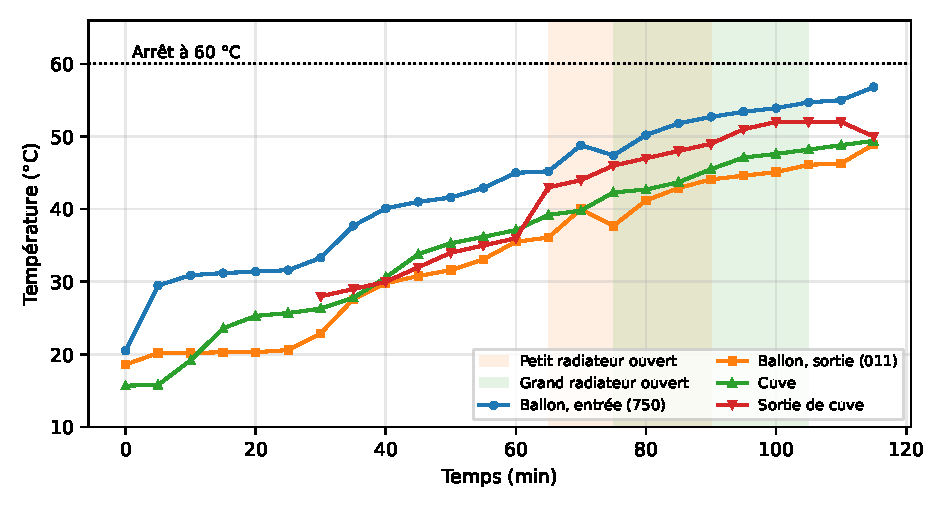
\includegraphics[width=0.9\textwidth]{Images/res_temp_ballon.pdf}
  \caption{Évolution des températures du ballon et de la cuve}
  \label{fig:temp-ballon}
\end{figure}

\paragraph{Radiateurs.} Les températures des radiateurs sont représentées à la figure~\ref{fig:temp-radiateurs}. Tant qu'ils sont fermés, elles restent à environ 20\,°C, soit la température ambiante au début de l'essai.
\begin{itemize}
  \item \emph{Grand radiateur}~: à l'ouverture (75~min), l'eau arrive à 45,6\,°C à l'entrée alors que la sortie n'est qu'à 27,3\,°C (écart de 18,3\,K), le radiateur étant encore froid. L'écart entre l'entrée et la sortie diminue ensuite de 4,8\,K (80~min) à 2,2\,K (100~min). L'entrée atteint 53,2\,°C à 105~min, puis les températures diminuent après la fermeture (42,9\,°C à l'entrée et 40,9\,°C à la sortie à 115~min).
  \item \emph{Petit radiateur}~: à l'ouverture (65~min), l'entrée est à 39,4\,°C et la sortie à 36,8\,°C (écart de 2,6\,K). Les deux températures montent ensuite ensemble jusqu'à environ 49\,°C à 90~min, avec des valeurs d'entrée et de sortie très proches, la sortie étant même légèrement supérieure à l'entrée (de 0,4 à 1,2\,K d'écart). Après la fermeture, elles redescendent jusqu'à 31,0\,°C à l'entrée et 31,5\,°C à la sortie à 115~min.
\end{itemize}

\begin{figure}[htbp]
  \centering
  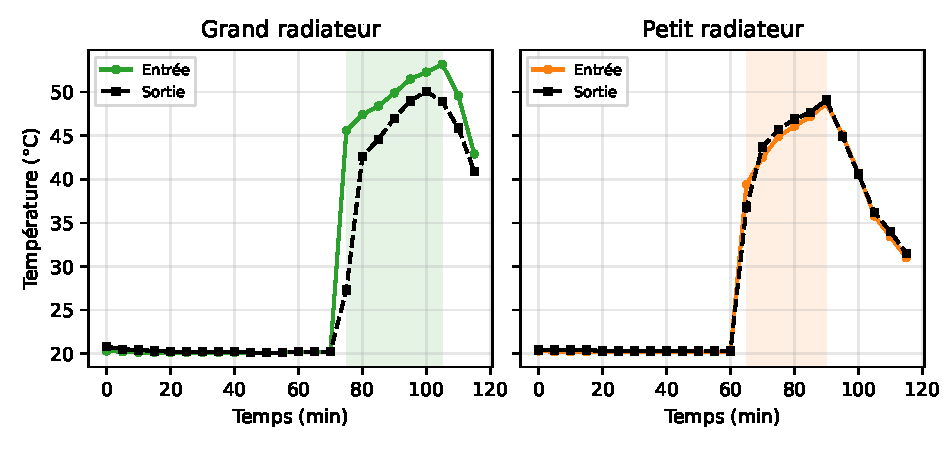
\includegraphics[width=0.95\textwidth]{Images/res_temp_radiateurs.pdf}
  \caption{Températures d'entrée et de sortie des radiateurs}
  \label{fig:temp-radiateurs}
\end{figure}

\subsection{Composition des fumées}
\label{subsec:res-fumees}

Les mesures de l'analyseur Testo~320 sont reprises à la figure~\ref{fig:fumees}. Au relevé initial, la cogénération étant à l'arrêt, l'analyseur indique 21\,\% d'O\textsubscript{2} et 0\,ppm de CO, et le CO\textsubscript{2} n'est pas affiché. En fonctionnement~:
\begin{itemize}
  \item la température des fumées passe de 66,3\,°C (5~min) à environ 70\,°C dès 10~min, puis reste comprise entre 70 et 73\,°C, avec une moyenne de 71,2\,°C~;
  \item la teneur en O\textsubscript{2} est stable à 8,0--8,1\,\% jusqu'à 60~min, puis devient plus variable, entre 8,1 et 11,1\,\%, avec une moyenne de 8,8\,\%~;
  \item la teneur en CO\textsubscript{2}, calculée par l'analyseur à partir de l'O\textsubscript{2}, évolue en sens inverse~: de 8,4\,\% au début, elle descend jusqu'à 6,4\,\%, avec une moyenne de 7,9\,\%~;
  \item la teneur en CO est comprise entre 393 et 588\,ppm, avec une moyenne de 486\,ppm~;
  \item la température ambiante augmente de 22,2 à 29,8\,°C.
\end{itemize}

\begin{figure}[htbp]
  \centering
  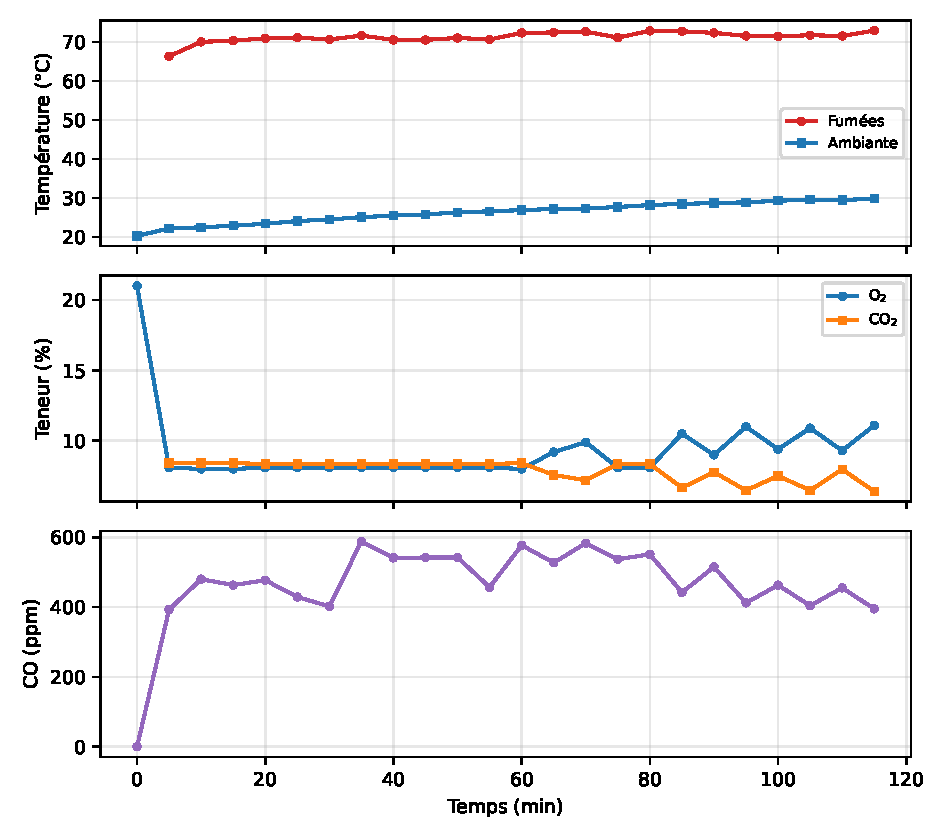
\includegraphics[width=0.9\textwidth]{Images/res_fumees.pdf}
  \caption{Mesures de l'analyseur de combustion Testo~320}
  \label{fig:fumees}
\end{figure}

\subsection{Consommation et production}
\label{subsec:res-puissances}

Les puissances sont déduites des relevés de compteurs et du système d'acquisition (section~\ref{sec:appareils}). Pour un pas de 5~minutes, avec $\Delta V$ la variation d'index du compteur de gaz (en m\textsuperscript{3}) et $\Delta E$ celle du compteur d'électricité (en kWh)~:
\begin{align}
  P_{\mathrm{gaz}} &= 12\,\Delta V \cdot \frac{\rho \cdot \mathrm{PCI}}{3600} \\
  P_{\mathrm{el}} &= 12\,\Delta E \\
  P_{\mathrm{th}} &= \frac{\text{Heat power}}{3{,}6}
\end{align}
avec $P_{\mathrm{gaz}}$, $P_{\mathrm{el}}$ et $P_{\mathrm{th}}$ en kW, et \emph{Heat power} la puissance thermique récupérée fournie par l'acquisition, en MJ/h. Pour le gaz naturel, nous avons pris une masse volumique $\rho$ de 0,7\,kg/m\textsuperscript{3} et un pouvoir calorifique inférieur PCI de 50\,MJ/kg (soit 35\,MJ/m\textsuperscript{3}, ou environ 9,7\,kWh/m\textsuperscript{3}).

Sur les 115~minutes de l'essai, la cogénération a consommé 4,442\,m\textsuperscript{3} de gaz (environ 43,2\,kWh), produit 10,59\,kWh d'électricité et récupéré environ 17,7\,kWh de chaleur. L'évolution des puissances est représentée à la figure~\ref{fig:puissances}~:
\begin{itemize}
  \item la puissance du gaz consommé est de 22,5\,kW en moyenne (de 17,4 à 26,5\,kW), pour un débit moyen de 2,32\,m\textsuperscript{3}/h~;
  \item la puissance thermique récupérée est stable, sans tendance au cours de l'essai, avec une moyenne de 9,2\,kW (de 8,3 à 10,4\,kW)~;
  \item la puissance électrique, déduite du compteur, varie davantage d'un relevé à l'autre, de 3,5 à 7,3\,kW, avec une moyenne de 5,5\,kW.
\end{itemize}
La puissance électrique de sortie (\emph{W out}) affichée par le système d'acquisition est quant à elle restée à 6\,000\,W à chaque relevé en fonctionnement.

\begin{figure}[htbp]
  \centering
  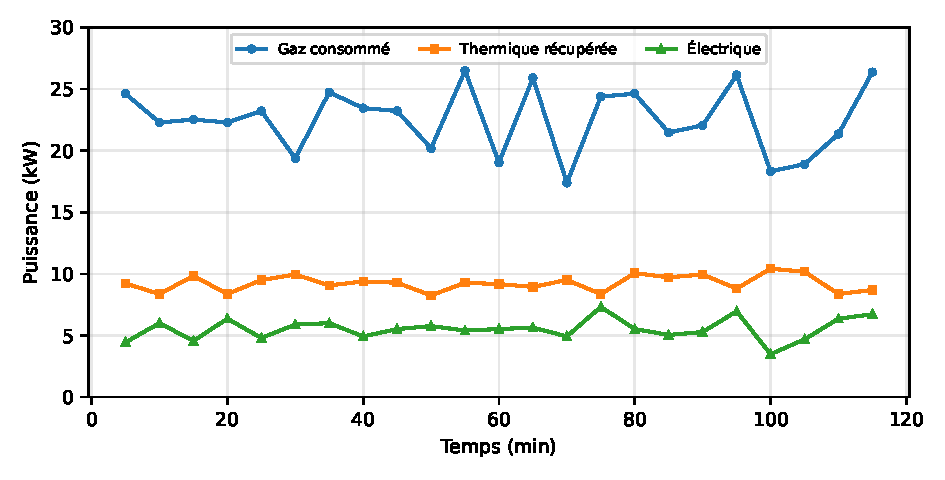
\includegraphics[width=0.9\textwidth]{Images/res_puissances.pdf}
  \caption{Puissances du gaz consommé, thermique récupérée et électrique}
  \label{fig:puissances}
\end{figure}

\subsection{Rendements}
\label{subsec:res-rendements}

Les rendements sont calculés pour chaque pas de 5~minutes, en rapportant les puissances électrique et thermique à celle du gaz consommé~:
\begin{equation}
  \eta_{\mathrm{el}} = \frac{P_{\mathrm{el}}}{P_{\mathrm{gaz}}}, \qquad
  \eta_{\mathrm{th}} = \frac{P_{\mathrm{th}}}{P_{\mathrm{gaz}}}, \qquad
  \eta_{\mathrm{global}} = \eta_{\mathrm{el}} + \eta_{\mathrm{th}}
\end{equation}
Leur évolution est représentée à la figure~\ref{fig:rendements} et leurs valeurs moyennes, sur les relevés de 5 à 115~min, sont reprises dans le tableau~\ref{tab:rendements}. Les valeurs instantanées fluctuent d'un relevé à l'autre, car elles dépendent de la variation d'index de compteurs relevés manuellement sur un pas de seulement 5~minutes.

\begin{table}[htbp]
  \centering
  \caption{Rendements mesurés (moyenne sur 5 à 115~min)}
  \label{tab:rendements}
  \begin{tabular}{lccc}
    \hline
    Rendement & Moyenne (\%) & Minimum (\%) & Maximum (\%) \\
    \hline
    Électrique & 24,7 & 18,0 & 30,4 \\
    Thermique & 41,8 & 33,0 & 56,9 \\
    Global & 66,4 & 55,4 & 83,0 \\
    \hline
  \end{tabular}
\end{table}

\begin{figure}[htbp]
  \centering
  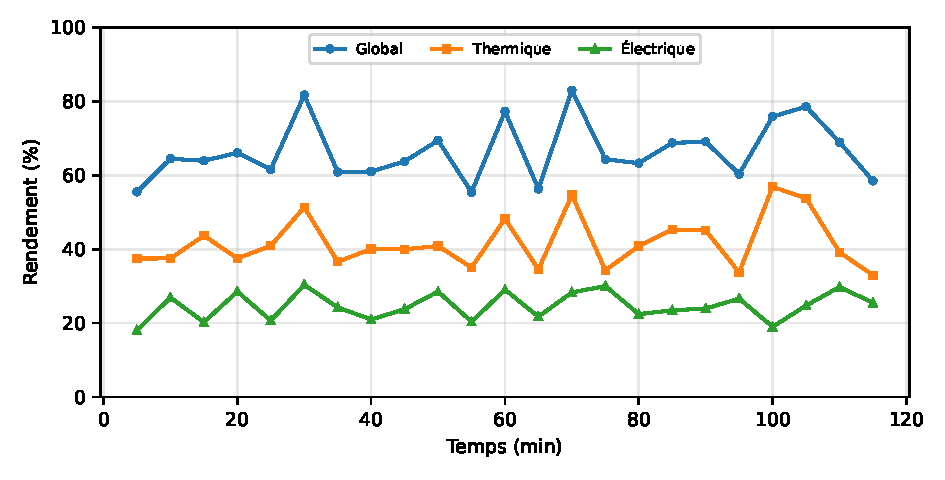
\includegraphics[width=0.9\textwidth]{Images/res_rendements.pdf}
  \caption{Évolution des rendements électrique, thermique et global}
  \label{fig:rendements}
\end{figure}

\section{Analyses}
\label{sec:analyses}

% Interprétation des résultats et comparaison avec les valeurs du constructeur.

% =====================================================================
% Chapitres 6 à 9 du rapport « Banc d'essai cogénération »
% À coller à la place des sections vides « Analyses », « Avantages »,
% « Inconvénients » et « Conclusion ».
%
% Paquets nécessaires : amsmath, graphicx, booktabs (+ url/hyperref
% pour la bibliographie). Les figures sont dans le dossier
% figures_analyse/ (à copier à côté du fichier .tex principal).
% Les références existantes [1] à [7] sont écrites en dur ; les
% nouvelles références (\cite{...}) sont à ajouter à la bibliographie
% (voir le bloc commenté à la fin de ce fichier).
% =====================================================================

Ce chapitre interprète les résultats du chapitre~5 et les compare aux
valeurs du constructeur (tableau~1). Sauf mention contraire, les
grandeurs sont calculées sur l'ensemble de l'essai (115~min), à partir
des variations d'index des compteurs et de la puissance thermique
fournie par le programme d'acquisition.

\subsection{Méthode : énergies cumulées plutôt que valeurs instantanées}
\label{sec:methode}

Les rendements du tableau~4 sont des moyennes de rapports calculés tous
les 5~minutes. Or ces rapports fluctuent fortement : le rendement global
instantané varie de 55,4 à 83,0~\%, alors que la puissance thermique
est quasi constante (de 8,3 à 10,4~kW). Cette dispersion vient du
fait que la puissance du gaz consommé varie de
17,4 à 26,5~kW alors qu'un moteur à régime stable ne devrait pas présenter de
telles variations. Chaque pas de 5~minutes ne correspond qu'à environ
0,2~m$^3$ de gaz : une incertitude d'une minute sur l'instant de lecture
du compteur manuel suffit à modifier la puissance de $\pm 20$~\%. Les
valeurs instantanées, y compris le maximum de 83~\% à 70~min, sont donc
des erreurs de mesure et non un fonctionnement réel proche des 85~\%
du constructeur.

Afin de s'affranchir de ce bruit, nous travaillons sur les énergies
cumulées sur la durée de l'essai :
\begin{equation}
  \eta_{\mathrm{el}} = \frac{E_{\mathrm{el}}}{E_{\mathrm{gaz}}},
  \qquad
  \eta_{\mathrm{th}} = \frac{Q_{\mathrm{th}}}{E_{\mathrm{gaz}}},
  \qquad
  \eta_{\mathrm{global}} = \eta_{\mathrm{el}} + \eta_{\mathrm{th}}
  \label{eq:rendements_cumules}
\end{equation}
avec $E_{\mathrm{gaz}} = \Delta V \cdot \rho \cdot \mathrm{PCI}/3{,}6$
(en kWh, avec $\rho \cdot \mathrm{PCI} = 35$~MJ/m$^3$),
$E_{\mathrm{el}}$ la variation d'index du compteur d'électricité et
$Q_{\mathrm{th}} = \sum_i P_{\mathrm{th},i} \cdot 5/60$ la chaleur
récupérée. Sur 115~minutes, la cogénération a consommé 43,2~kWh de gaz
(4,442~m$^3$), produit 10,59~kWh d'électricité et récupéré 17,7~kWh de
chaleur, soit :
\begin{equation}
  \eta_{\mathrm{el}} = 24{,}5~\%, \qquad
  \eta_{\mathrm{th}} = 41{,}0~\%, \qquad
  \eta_{\mathrm{global}} = 65{,}5~\%
\end{equation}
Ces valeurs sont proches des moyennes du tableau~4 (24,7~\%, 41,8~\%
et 66,4~\%), mais elles sont moins sensibles aux erreurs de lecture.
La figure~\ref{fig:cumul} montre que les trois énergies cumulées évoluent
linéairement avec le temps, ce qui confirme un régime stable dès les
premières minutes.

\begin{figure}[htbp]
  \centering
  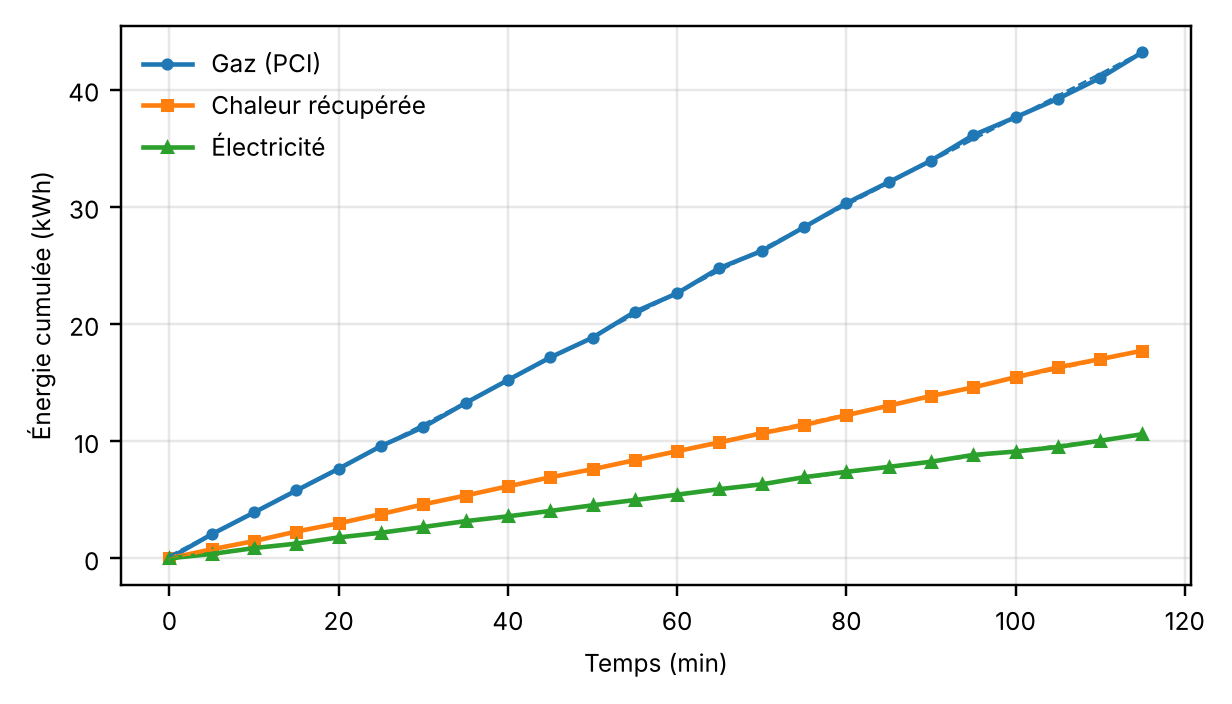
\includegraphics[width=0.9\textwidth]{figures_analyse/fig_energies_cumulees.png}
  \caption{Énergies cumulées (gaz, chaleur récupérée, électricité)}
  \label{fig:cumul}
\end{figure}

\subsection{Comparaison avec les valeurs du constructeur}
\label{sec:comparaison}

Le tableau~\ref{tab:comparaison} compare les valeurs mesurées à celles
du constructeur (tableau~1).

\begin{table}[htbp]
  \centering
  \caption{Valeurs mesurées (énergies cumulées sur 115~min) et valeurs du constructeur}
  \label{tab:comparaison}
  \begin{tabular}{lccc}
    \toprule
    Grandeur & Constructeur & Mesuré & Écart \\
    \midrule
    Puissance du gaz (kW)          & 20,8 & 22,5 & $+8$~\% \\
    Puissance électrique (kW)      & 6,0  & 5,5  & $-8$~\% \\
    Puissance thermique (kW)       & 11,7 & 9,2  & $-21$~\% \\
    Rendement électrique (\%)      & 28,8 & 24,5 & $-4{,}3$ points \\
    Rendement thermique (\%)       & 56,2 & 41,0 & $-15{,}2$ points \\
    Rendement global (\%)          & 85,0 & 65,5 & $-19{,}5$ points \\
    \bottomrule
  \end{tabular}
\end{table}

Le rendement global mesuré est inférieur de près de 20 points à celui du
constructeur. Cet écart se répartit entre une baisse de 4,3~points sur
le rendement électrique et de 15,2~points sur le rendement thermique.
Plusieurs éléments permettent de nuancer ou d'expliquer ces écarts.

\paragraph{Puissance du gaz.} La puissance du gaz dépend du produit
$\rho \cdot \mathrm{PCI}$ supposé, qui est une valeur générique, et du
volume lu au compteur, qui n'est pas corrigé en pression et en
température. Le pouvoir calorifique réel du gaz distribué (indiqué par
le gestionnaire de réseau ou sur une facture) peut s'écarter de
quelques pour cent de notre hypothèse. La valeur du constructeur est donnée dans des conditions de
référence (100~kPa, 25~°C, 30~\% d'humidité) et la base de calcul
(PCI ou PCS) n'est pas précisée dans [3] ; elle devrait être vérifiée,
car un rendement exprimé sur PCS serait inférieur d'environ 10~\% à un
rendement exprimé sur PCI.

\paragraph{Puissance électrique.} La puissance électrique de sortie
(\emph{W out}) affichée par le logiciel d'acquisition reste exactement à 6\,000~W à chaque
relevé : une valeur aussi constante est probablement une consigne ou une
valeur nominale affichée plutôt qu'une mesure. À 6~kW, l'unité aurait
produit 11,5~kWh en 115~min, contre 10,59~kWh lus au compteur
(soit $-8$~\%). Nous retenons donc la valeur du
compteur (5,5~kW en moyenne), plus fiable. Elle est plus cohérente, notamment avec le
premier pas de 5~min qui a une moyenne 4,4~kW, ce qui correspondrait à la montée en puissance
au démarrage.

\paragraph{Puissance thermique.} La puissance thermique récupérée
(9,2~kW) est inférieure de 21~\% à celle du constructeur. L'écart ne
s'explique pas par la température d'entrée de l'eau : le constructeur
raisonne avec un retour à 60~°C, alors que celui de notre essai se situe
entre 20 et 49~°C, ce qui favorise plutôt l'échange avec le liquide de
refroidissement. Le débit n'a pas été mesuré, mais il peut être estimé à
partir de l'écart de température entre l'entrée et la sortie du ballon
(7,9 à 11,1~°C, moyenne de 9,6~°C) :
\begin{equation}
  \dot{m} = \frac{P_{\mathrm{th}}}{c_p \,\Delta T}
  \approx \frac{9{,}2}{4{,}186 \times 9{,}6} \approx 0{,}23~\mathrm{kg/s}
  \approx 14~\mathrm{L/min}
\end{equation}
Cette estimation (de 11 à 17~L/min selon le relevé) suppose que la
puissance thermique de l'acquisition est correcte ; elle ne peut donc
pas la valider. Elle indique toutefois que le débit réel était nettement
inférieur aux 34,1~L/min du constructeur : avec 34,1~L/min et un écart
de 9,6~K, la puissance serait de 22~kW, soit toute la puissance du gaz
consommé, ce qui est impossible. Notre essai ne s'est donc déroulé ni
au débit ni à la température de retour de référence, et les écarts du
tableau~\ref{tab:comparaison} ne sont pas comparables au
point de fonctionnement du constructeur. Pour une exploitation correcte,
il faudrait mesurer le débit d'eau sortant de la machine lors
d'un prochain essai.

\subsection{Bilan énergétique et pertes}
\label{sec:bilan}

La figure~\ref{fig:bilan} compare la répartition de l'énergie du gaz (énergie consommée)
selon le constructeur et selon notre essai. Les pertes passent de
15,0~\% à 34,5~\%.

\begin{figure}[htbp]
  \centering
  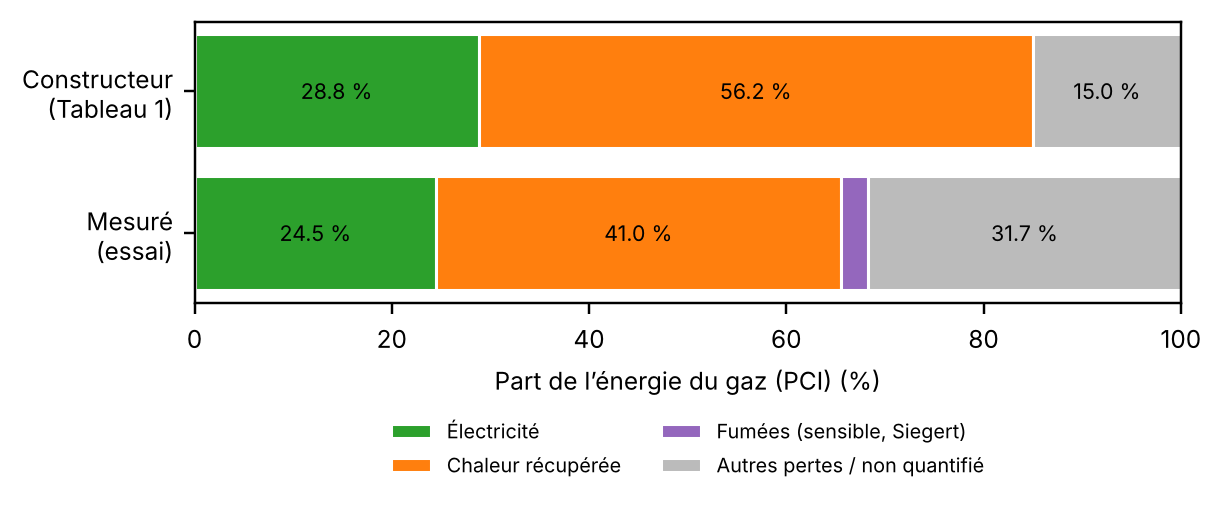
\includegraphics[width=0.9\textwidth]{figures_analyse/fig_bilan_energetique.png}
  \caption{Répartition de l'énergie du gaz (base PCI) : valeurs du
  constructeur et valeurs mesurées}
  \label{fig:bilan}
\end{figure}

Parmi ces pertes, nous pouvons en quantifier deux à partir de
l'analyseur de combustion :
\begin{itemize}
  \item \emph{la chaleur sensible des fumées}, par la formule de
  Siegert $q_A = (T_{\mathrm{fum}} - T_{\mathrm{amb}}) \left(\frac{A_2}{21 - \mathrm{O}_2} + B\right)$,
  avec les coefficients usuels du gaz naturel ($A_2 = 0{,}66$ et
  $B = 0{,}009$). Avec un écart de température de 45~°C environ et
  8,8~\% d'O$_2$, on obtient $q_A \approx 2{,}8$~\% (0,64~kW) ;
  \item \emph{le CO imbrûlé}, dont la combustion libérerait environ
  0,2~\% de l'énergie du gaz (calcul à partir du rapport
  $\mathrm{CO}/(\mathrm{CO} + \mathrm{CO}_2)$ et des pouvoirs
  calorifiques du CO et du méthane).
\end{itemize}
Ces deux postes ne représentent que 3~\% de l'énergie du gaz : les
fumées ne sont donc pas la cause principale de l'écart. Il reste
environ 31,5~\% d'énergie non expliquée, contre 15~\% pour le
constructeur. Elle regroupe plusieurs postes que nos mesures ne
permettent pas de séparer : les pertes du générateur et de l'onduleur,
la chaleur cédée à l'air de l'armoire par le moteur et le circuit de
refroidissement, un
éventuel passage dans le radiateur interne (section~2.2), les
hydrocarbures imbrûlés d'un moteur à mélange pauvre (non mesurés), et
enfin les erreurs sur le pouvoir calorifique et sur la puissance
thermique de l'acquisition.

\subsection{Circuit hydraulique et radiateurs}
\label{sec:hydraulique}

\paragraph{Vitesse d'échauffement.} Les pentes de température du ballon
sont reprises dans le tableau~\ref{tab:pentes}. Elles diminuent au fur
et à mesure que l'essai avance, alors que la puissance thermique reste
constante : l'ouverture des radiateurs (à partir de 65~min) et les
pertes thermiques croissantes de la cuve absorbent une part de plus en
plus grande de la chaleur.

\begin{table}[htbp]
  \centering
  \caption{Vitesse d'échauffement de l'eau du ballon (K/min)}
  \label{tab:pentes}
  \begin{tabular}{lccc}
    \toprule
    Fenêtre (min) & Entrée du ballon & Sortie du ballon (retour) & Radiateurs \\
    \midrule
    30 à 60  & 0,34 & 0,36 & fermés \\
    60 à 90  & 0,27 & 0,29 & ouverts \\
    90 à 115 & 0,15 & 0,17 & ouverts puis fermés \\
    \bottomrule
  \end{tabular}
\end{table}

\paragraph{Capacité thermique équivalente et bilan de chaleur.}
Entre 30 et 60~min, les radiateurs sont fermés et la quasi-totalité de
la chaleur récupérée (9,1~kW en moyenne) sert à chauffer l'eau, dont la
température moyenne (moyenne de l'entrée et de la sortie du ballon)
augmente de 0,41~K/min. On en déduit une capacité thermique équivalente
d'environ 1\,340~kJ/K, soit l'équivalent de 320~kg d'eau. Une seconde
estimation est possible : le front d'eau froide atteint la sortie du
ballon vers 27~min ; à un débit de 14~L/min, cela correspond à un
volume d'environ 380~L. Les deux ordres de grandeur sont cohérents
(300 à 400~L) et sont à comparer au volume réel de la cuve, qui n'a pas
été relevé.

En conservant cette capacité thermique, on estime la part de chaleur
qui n'est pas stockée (tableau~\ref{tab:bilan_cuve}). Elle correspond à
la chaleur dissipée par les radiateurs et par les pertes de la cuve.

\begin{table}[htbp]
  \centering
  \caption{Bilan de chaleur de la cuve (estimation)}
  \label{tab:bilan_cuve}
  \begin{tabular}{lccc}
    \toprule
    Fenêtre (min) & $P_{\mathrm{th}}$ (kW) & Stockée (kW) & Radiateurs et pertes (kW) \\
    \midrule
    60 à 90  & 9,4 & 6,1 & 3,3 \\
    90 à 115 & 9,3 & 4,0 & 5,3 \\
    \bottomrule
  \end{tabular}
\end{table}

Sur l'ensemble de la période de 30 à 115~min, environ 70~\% de la
chaleur récupérée (9,2 sur 13,1~kWh) est stockée dans l'eau, et 30~\%
est dissipée. Pour comparer, si tout le débit estimé (0,23~kg/s)
traversait le grand radiateur, son écart de température de 2,2 à 4,8~K
correspondrait à une puissance de 2,1 à 4,6~kW, ce qui est du même ordre
de grandeur que les valeurs du tableau~\ref{tab:bilan_cuve}. Ce bilan
reste toutefois une estimation, car il repose sur un débit non mesuré
et sur des sondes dont la précision est de $\pm 1{,}3$~K.

\subsection{Composition des fumées}
\label{sec:fumees}

\paragraph{Excès d'air.} À partir de la teneur en O$_2$, le coefficient
d'excès d'air $\lambda = 21/(21 - \mathrm{O}_2)$ vaut 1,74 en moyenne
(de 1,62 à 2,12). Le moteur fonctionne donc bien en mélange pauvre,
comme annoncé à la section~3.1.

\paragraph{Vérification du CO$_2$.} L'analyseur ne mesure pas le CO$_2$ :
il le calcule à partir de l'O$_2$ et du CO$_2$ maximal du combustible
sélectionné. Les valeurs de l'annexe (8,42~\% pour 8,0~\% d'O$_2$)
correspondent à un CO$_2$ maximal d'environ 13,6~\%, alors qu'il vaut
environ 11,9~\% pour le gaz naturel. Avec cette dernière valeur, le CO$_2$
serait de 6,9~\% en moyenne (de 5,6 à 7,4~\%) au lieu de 7,9~\%. Il est
donc probable que l'analyseur n'était pas réglé sur le gaz naturel. Cela
n'affecte pas l'O$_2$ ni le CO, mesurés directement, mais le CO$_2$ que nous avons mesuré est très probablement faux.

\paragraph{Niveau de CO.} Le CO est compris entre 393 et 588~ppm (moyenne
de 486~ppm), soit un écart bien supérieur à la précision de l'appareil
($\pm 20$~ppm ou $\pm 5$~\%) : les variations sont réelles. Pour comparer
des mesures à des teneurs en O$_2$ différentes, on ramène le CO à une
teneur de référence :
\begin{equation}
  \mathrm{CO}_{\mathrm{ref}} = \mathrm{CO} \cdot \frac{21 - \mathrm{O}_{2,\mathrm{ref}}}{21 - \mathrm{O}_2}
\end{equation}
Ramené à 0~\% d'O$_2$, le CO vaut 842~ppm en moyenne (de 640 à 1\,100~ppm).
La figure~\ref{fig:co} montre que la baisse apparente du CO après
60~min (de 491 à 480~ppm en moyenne) accompagne la hausse de l'O$_2$ (de
8,1 à 9,7~\% en moyenne) : c'est un effet de dilution. Ramené à 0~\%
d'O$_2$, le CO augmente même de 798 à 890~ppm entre les deux périodes.
La combustion ne s'est donc pas améliorée. L'oscillation de l'O$_2$
après 60~min coïncide avec l'ouverture des radiateurs, mais nos mesures
ne permettent pas d'établir un lien.

\begin{figure}[htbp]
  \centering
  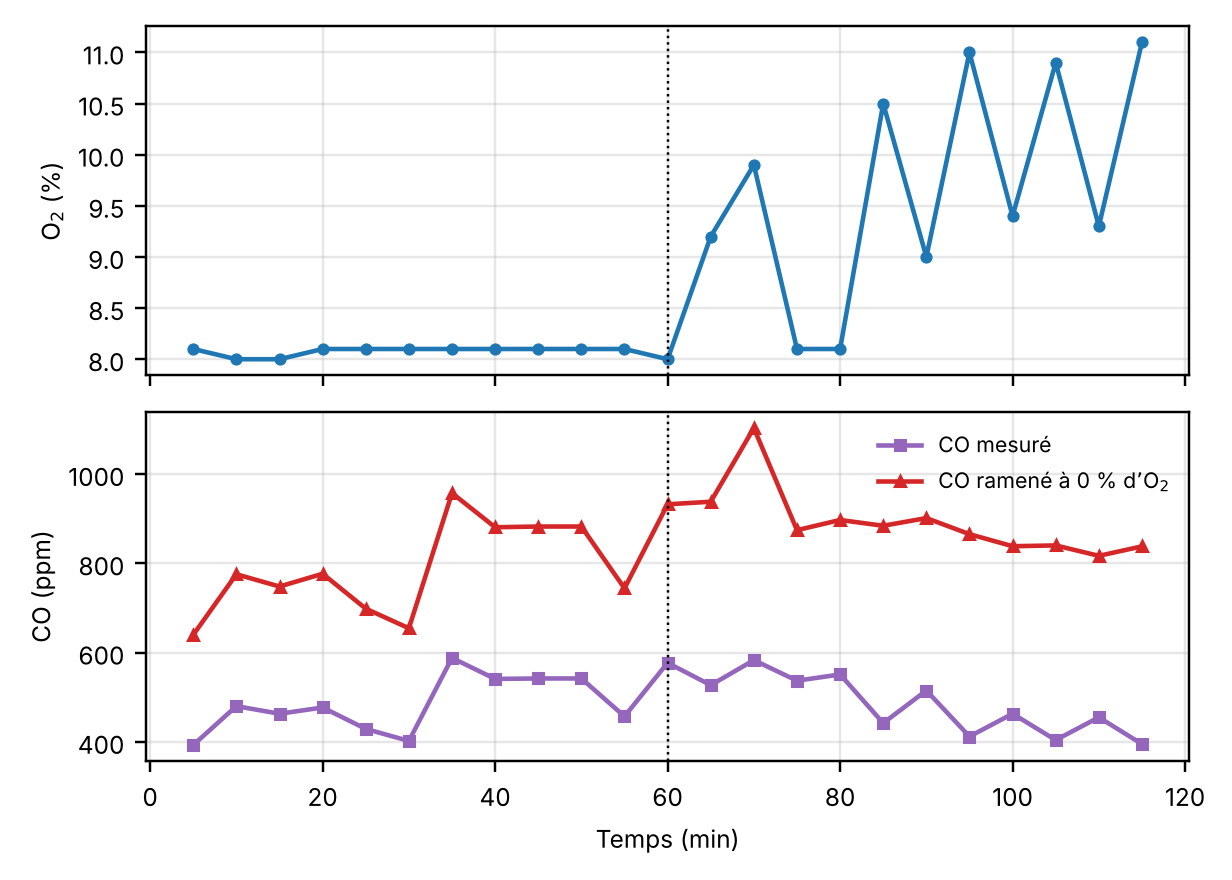
\includegraphics[width=0.85\textwidth]{figures_analyse/fig_co_normalise.png}
  \caption{Teneur en O$_2$ (haut), CO mesuré et CO ramené à 0~\% d'O$_2$
  (bas). La ligne en pointillés marque 60~min.}
  \label{fig:co}
\end{figure}

\paragraph{Repères sur les niveaux de CO.} Les seuils d'exposition
usuels (de l'ordre de 35~ppm sur 8~heures, 200~ppm sur 15~minutes et
1\,200~ppm pour un danger immédiat pour la vie [1]) sont largement
dépassés par les gaz d'échappement : l'évacuation des fumées vers
l'extérieur par la conduite de ventilation (figure~2) est donc
indispensable. Pour les émissions, la Région de Bruxelles-Capitale
impose aux moteurs au gaz naturel neufs de cogénération de 20~kW et plus
une valeur limite de 112,5~mg/Nm$^3$ de CO à 15~\% d'O$_2$
\cite{bxl_cogeneration}. Notre mesure convertie dans les mêmes
conditions (1~ppm de CO $=$ 1,25~mg/Nm$^3$) vaut environ 300~mg/Nm$^3$,
soit 2,7 fois cette limite (environ 800~mg/Nm$^3$ à 5~\% d'O$_2$). Cette
limite montre que la cogen de l'école n'est pas au
niveau des exigences actuelles. Nous n'avons pas mesuré les NO$_x$.

\subsection{Économie d'énergie primaire}
\label{sec:pes}

Pour juger l'intérêt énergétique d'une cogénération, on compare le gaz
consommé à celui qui serait nécessaire pour produire séparément la même
électricité (dans une centrale) et la même chaleur (dans une chaudière).
L'économie d'énergie primaire est
\begin{equation}
  \mathrm{PES} = 1 - \frac{1}{\dfrac{\eta_{\mathrm{th}}}{\eta_{\mathrm{ref,th}}} + \dfrac{\eta_{\mathrm{el}}}{\eta_{\mathrm{ref,el}}}}
  \label{eq:pes}
\end{equation}
Nous prenons pour le gaz naturel des rendements de référence de 52,5~\%
pour l'électricité et de 90~\% pour la chaleur, d'après le règlement
délégué (UE) 2015/2402 \cite{reglement_ref}. Les valeurs exactes
dépendent de l'année de construction de l'unité, et nous n'appliquons
pas le facteur de correction lié aux pertes de réseau évitées. Pour une
cogénération de moins de 1~MW électrique, la directive 2012/27/UE exige
une économie positive. Les résultats sont :
\begin{itemize}
  \item avec les valeurs du constructeur ($\eta_{\mathrm{el}} = 28{,}8$~\%
  et $\eta_{\mathrm{th}} = 56{,}2$~\%) : $\mathrm{PES} = +14{,}7$~\% ;
  \item avec nos valeurs mesurées ($\eta_{\mathrm{el}} = 24{,}5$~\%
  et $\eta_{\mathrm{th}} = 41{,}0$~\%) : $\mathrm{PES} = -8{,}4$~\%.
\end{itemize}
À performances mesurées, la cogénération consomme donc plus de gaz que
la production séparée. Pour atteindre une économie nulle avec notre
rendement électrique, il aurait fallu un rendement thermique d'au moins
48~\%. Ce résultat dépend du fonctionnement au point nominal, et il suppose
que toute la chaleur produite est utilisée.

\section{Avantages}
\label{sec:avantages}
Dans cette section, nous allons détaillé les avantages lié à cette unité de cogénération. Nous allons séparer ce chapitre en deux partie. La partie économique puis la partie environnementales.
\subsection{Avantages économiques}
\label{subsec:avantages-eco}
Etant donné que nous faisons tourner un moteur qui lui-même fait tourner un alternateur, le principale avantage de cette untié est qu'elle produit de l'électricité.
Cela veut dire que nous pouvons produire de l'électricité a peu près sur commande ce qui signifie que nous pouvons diminuer la consommation de l'électricité du réseaux lorsque le prix de celle-ci est en hausse.
Ensuite, suite aux normes du pays, nous pouvons obtenir éventuellement des subvention pour nous aider à acheter ce type de machine.

\subsection{Avantages environnementaux}
\label{subsec:avantages-env}
Ce système permet de récupérer la chaleur produite par le moteur, qui, en temps normal, est entièrement perdue. En effet, lorsque le moteur chauffe, 
nous récupérons cette énergie afin de chauffer un réservoir d'eau. Ce qui a pour avantage de pouvoir avoir de l'eau chaude "gratuitement" alors qu'en temps normal,
nous aurions dû avoir une machine qui consomme aussi de l'énergie fossile pour faire chauffer cette eau.
Nous réduisosns donc les émission de GES en utilisant cette unité.

\section{Inconvénients}
\label{sec:inconvenients}
Dans cette section, nous allons détaillé les inconvénients lié à cette unité de cogénération.
Malheureusement il y a quelques inconvénient non négligeable à connaître et à pointer :
\begin{enumerate}
  \item Le prix du carburant que le moteur utilise (ici c'est du gaz). Ce prix est amené à beaucoup fluxctuer et peu devenir très cher (comme maintenant). Ce qui pose un réel problème quand au gain global de cette unité.
  \item L'entretient doit être régulier et à un coût élevé
  \item La durée de vie est assez courte (10  à 15 ans)
  \item Il faut une installation qui accompagne cette machine. En effet, il faut un circuit de chauffage particulier et on ne peut pas générer de l'électricité directement sur le réseaux aussi facilement.
  \item Si nous n'avons pas besoin de chauffage (comme en été), l'unité perd une grande partie de ses avantages.
\end{enumerate}

\section{Conclusion}
\label{sec:conclusion}
Cet essai de 115~minutes sur une micro-cogénération au gaz naturel
(6~kW électriques nominaux) nous permet de comprendre les principes de la cogénération, mais
l'installation n'atteint pas les performances annoncées. Calculé sur les
énergies cumulées, le rendement global est de 65,5~\% (24,5~\%
électrique et 41,0~\% thermique), contre 85~\% pour le constructeur. La
puissance thermique récupérée (9,2~kW) est inférieure de 21~\% à la
valeur nominale, et le débit estimé (environ 14~L/min au lieu de
34,1~L/min).

À performances mesurées, l'économie d'énergie primaire est négative
($-8{,}4$~\%, contre $+14{,}7$~\% avec les valeurs du constructeur,
section~\ref{sec:pes}). L'intérêt d'une telle unité dépend donc d'un
fonctionnement proche du point nominal, que la machine ne sait pas atteindre dans son état actuel, d'un besoin de chaleur régulier et
d'un rapport favorable entre les prix de l'électricité et du gaz.
 
Ilserait intéressant de réaliser un nouvel essai avec le débit
d'eau mesuré afin de connaitre la puissance thermique réellement récupérée.

\section{Bibliographie}
\label{sec:bibliographie}

\begin{thebibliography}{9}
  \bibitem{msss} « Barèmes utilisés par les organismes publics -- Monoxyde de carbone -- Professionnels de la santé -- MSSS ». Consulté le : 7 novembre 2026. [En ligne]. Disponible sur : \url{https://msss.gouv.qc.ca/professionnels/sante-environnementale/monoxyde-de-carbone/baremes-utilises-par-les-organismes-publics}
  \bibitem{picbleu} « Cogénération, minicogénération et microcogénération ». Consulté le : 7 novembre 2026. [En ligne]. Disponible sur : \url{https://picbleu.fr/les-articles/cogeneration-minicogeneration-et-microcogeneration}
  \bibitem{mchp} AISIN, \emph{MCHP Service Manual draft}. Document fourni dans le cadre du cours (UE06 HVAC, TP~6 Cogénération).
  \bibitem{desc} \emph{Descriptions des éléments de la machine}. Photographies annotées de l'installation, document fourni dans le cadre du cours (UE06 HVAC, TP~6 Cogénération).
  \bibitem{acq} AISIN, \emph{Operation manual of the maintenance checker (GEC Monitor)}, 2006. Document fourni dans le cadre du cours sous le titre «~Manuel d'utilisation du programme d'acquisition~» (UE06 HVAC, TP~6 Cogénération).
  \bibitem{testo115i} Testo, \emph{testo 115i -- Thermomètre à pince piloté par smartphone}, fiche technique 1982 1844/TT/08.2024. Consulté le : 7 novembre 2026.
  \bibitem{testo320} Testo, \emph{testo 320 -- Analyseur de combustion standard}, fiche technique 0981 2884/af/dk/05.2026. Consulté le : 7 novembre 2026.
  \bibitem{reglement_ref} Commission européenne, \emph{Règlement délégué (UE) 2015/2402 de la Commission du 12 octobre 2015 réexaminant les valeurs de rendement de référence harmonisées pour la production séparée d'électricité et de chaleur}, modifié par le règlement délégué (UE) 2023/2104. Consulté le : 7 novembre 2026. [En ligne]. Disponible sur : \url{https://eur-lex.europa.eu/eli/reg_del/2015/2402/oj}
  \bibitem{testachats_nov} Test-Achats, « Cartes tarifaires novembre 2026 ». Consulté le : 7 novembre 2026. [En ligne]. Disponible sur : \url{https://www.test-achats.be/maison-energie/gaz-electricite-mazout-pellets/presse/cartes-tarifaires-novembre-2026}
  \bibitem{co2_reseau} Université de Liège (ORBi), \emph{Belgian grid emission factors 1950--2050}, 2026. Consulté le : 7 novembre 2026. [En ligne]. Disponible sur : \url{https://orbi.uliege.be/handle/2268/345758}
  \bibitem{ipcc} GIEC, \emph{2006 IPCC Guidelines for National Greenhouse Gas Inventories}, vol.~2 « Energy », chap.~2, facteur d'émission par défaut du gaz naturel (56,1~kg CO$_2$/GJ).
  \bibitem{bxl_cogeneration} Région de Bruxelles-Capitale, arrêté du 26 novembre 2020 fixant des conditions d'exploitation applicables aux installations de cogénération, valeurs limites reprises dans la décision de permis d'environnement PE~158/2019 (commune d'Anderlecht). Consulté le : 7 novembre 2026. [En ligne]. Disponible sur : \url{https://anderlecht.be/sites/default/files/medias/Files/environnement/2024/}
\end{thebibliography}



\section{Annexes}
\label{sec:annexes}

\subsection{Valeurs collectées}
\label{subsec:valeurs}

\end{document}